% The entire content of this work (including the source code
% for TeX files and the generated PDF documents) by 
% Hongxiang Chen (nicknamed we.taper, or just Taper) is
% licensed under a 
% Creative Commons Attribution-NonCommercial-ShareAlike 4.0 
% International License (Link to the complete license text:
% http://creativecommons.org/licenses/by-nc-sa/4.0/).
\documentclass{article}

\usepackage{float}  % For H in figures
\usepackage{amsmath} % For math
\usepackage{amssymb}
\numberwithin{equation}{subsection} % have the enumeration go to the subsection level.
									% See:https://en.wikibooks.org/wiki/LaTeX/Advanced_Mathematics
\usepackage{graphicx}   % need for figures
\usepackage{cite} % need for bibligraphy.
\usepackage{hyperref}  % make every cite a link
\usepackage{CJKutf8} % For Chinese characters
\usepackage{fancyref} % For easy adding figure,equation etc in reference. Use \fref or \Fref instead of \ref
\usepackage{braket} %http://tex.stackexchange.com/questions/214728/braket-notation-in-latex

% Following is for theorems etc environments
% http://tex.stackexchange.com/questions/45817/theorem-definition-lemma-problem-numbering && https://en.wikibooks.org/wiki/LaTeX/Theorems
\usepackage{amsthm}
\newtheorem{thm}{Theorem}
\newtheorem{lemma}{Lemma}


\title{%
	Feynman Diagram \\
	\large Part I - Interaction Picture}
\date{\today}
\author{Taper}


\begin{document}


\maketitle
\tableofcontents

\begin{abstract}
In this article, we introduces the basic Interaction Picture in quantum mechanics, then introduce the idea of "adiabatic turn on", which is supported by Gell-Mann and Low theorem (proved in appendix). 

% Next we define the Green function and provide three reasons for studying Green functions. Finally, we provide a few remarks on other types of Green functions, and on how Green functions, combined with Wick's theorem, lead to the development of Feynman Diagrams. 

\end{abstract}

\section{Note}
This note is intended for learning Feynman Diagram techniques in many-body physics. However, due to the limited time and the growing size of this document, I have to split it into small parts. This first part provides one foundational material for the beginning of Feynman Diagrams, i.e. Interaction Picture of quantum mechanics. Further updates will be found on my blog\cite{blog} within this summer vocation.

The style of the article might be fastidious. Yet I have try to maintain some physical viewpoints. Also, I will provide readers with reference to original materials whenever possible.

\section{Natural Units}

For convenience, I will use the unit system s.t. $\hbar=1$. An example of such unit systems is Plank units. 
\footnote{Readers could refer to \cite{wiki:Plank_units} for details.} Usually, calculation down in such unit systems are carried out mathematically first, then those normalized (being set to $1$) units, such as $\hbar$ here, are inserted back to the equations by dimensional analysis. For example, in this article when one sees the imaginary unit $i$, one should replace it with $\frac{i}{\hbar}$ or sometimes $i\hbar$ to get back to S.I. units.

\section{Interaction Picture}

The Interaction Picture
    \footnote{This part follows much of section 6 of \cite{fetter}. Similar material could also be found on section 2.1 of \cite{mahan}.}
is a very important way to view physical systems as interacting systems growing from the underlying ground state systems. In Interaction Picture,
both the wave functions and the operators are time dependent. The Hamiltonian is separated into the ground state part and the interaction part:
	$$H=H_0+V$$
where
	\begin{itemize}
		\item 		$H_0:$
		is taken to be an exactly solvable Hamiltonian. Note that $H_0$ should be bilinear in $C^{\dagger}\text{ and } C$ for Wick's theoren to be applicable.
		\footnote{See page 79, Sec 2.4 of \cite{mahan}}
	\end{itemize}

The operators and states are related to Schrödinger's Picture by
		
\begin{align}
	\ket{\Psi_I} &=  e^{iH_0t} \ket{\Psi_s}= e^{iH_0t}e^{-iHt} \ket{ \Psi_H} \label{eq:def_Psi}  	\\
	\hat{O}_1 &= e^{iH_0t}\hat{O}_Se^{-iH_0t}
\end{align}
	
where subscripts denoting:
	\begin{itemize}
		\item 		I:Interaction Picture
		\item		S: Schrödinger Picture
		\item		H: Heisenberg Picture
	\end{itemize}
	
Remark: we see that the "inner product" value is unaltered by this:
	$$\braket{\Psi_I|\hat{O}_S|\Psi_S} 
	= \braket{\Psi_S|e^{-iH_0t} \cdot (e^{iH_0t}\Hat{O}e^{-iH_0t}) \cdot e^{iH_0t}|\Psi_S }
	=\braket{\Psi_S|\Hat{O}_S|\Psi_S}$$
Physically, this leaves the probabilities (the only important value) unchanged.

The evolution of states is governed by equation of motion. In Schrödinger Picture, it is the Schrödinger's equation. In Interaction Picture, we will mainly deal the evolution operator.

	\subsection{Equation of Motion for Observables}
	
	Before we talk about evolution operator, we mention two useful results. The first is a equation of motion for observables in Interaction Picture.
	
	Since: $\hat{O}_I(t) = e^{i\hat{H_0}t}\hat{O}_S e^{-i\hat{H}_0t}$, we have:
	\begin{align}
		& i\cdot \frac{\partial \hat{O}_I(t)}{\partial t}\nonumber\\
		&= i\left[  i\hat{H}_0 e^{i\hat{H_0}t} \hat{O}_S e^{-i\hat{H_0}t}] + e^{i\hat{H_0}t} \hat{O}_S(-i\hat{H}_0) e^{-i\hat{H_0}t} \right]\nonumber\\
		&= -\hat{H}_0 (e^{i\hat{H_0}t} \hat{O}_S e^{-i\hat{H_0}t})
			+ e^{i\hat{H_0}t}\hat{O}_Se^{-i\hat{H_0}t} \hat{H}_0 \nonumber\\
		&= [\hat{O}_I(t),\hat{H}_0]
	\end{align}
	This looks very similar to the Heisenberg's equation, which is reasonable since in both pictures the operators is time-dependent.
	
	\subsection{Equation of Motion for wave function}
	
	Another important result is the following equation:
		
	\begin{align}
	i \frac{\partial}{\partial t} \ket{\Psi_I(t)} 
	=& i \frac{\partial}{\partial t} (e^{i\hat{H}_0t} \ket{\Psi_S(t)})
	\\
	=& i (i\hat{H}_0)\cdot \ket{\Psi_I(t)} + e^{i\hat{H}_0t} \cdot \frac{\partial}{\partial t} \ket{\Psi_S(t)}
	\\
	=& -\hat{H}_0 \ket{\Psi_I(t)} + e^{i\hat{H}_0t} (H_0+V) \ket{\Psi_S(t)}
	\\
	=& [-\hat{H}_0 + e^{iH_0t} (\hat{H}_0 +V) e^{-i\hat{H}_0t}] \ket{\Psi_I(t)}
	\\
	\label{eq:motion} =& \hat{V}_I \ket{\Psi_I(t)}		
	\end{align}
	
	
	However, in Interaction Picture, there is one operator which is even more important than the above equations. It is the evolution operator to be defined below.
	
	\subsection{The evolution operator in Interaction picture}
	
	\textbf{Note:} From now on, we work mostly in Interaction Picture. Hence the subscript $I$ will be neglected, when it is convenient, for operators or states in Interaction Picture.
	
	The evolution operator $\hat{U}(t,t_0)$ is defined s.t. 
	\begin{align}\ket{\Psi(t)}= \hat{U}(t,t_0) \ket{\Psi (t_0)}\end{align}
	
	We observe that $\hat{U}$ behaves just like the time-evolution operator in Schrödinger Picture: it brings a state at time $t_0$ to a later time $t$. For finite time, it can be given a formal expression as follows:
	
	By \fref{eq:def_Psi} we have
	\begin{align}
    	\ket{\Psi_I(t)} &= e^{iH_0t} \ket{\Psi_S(t)}
    	\\
    	&= e^{iH_0t}\cdot e^{iH(t-t_0)} \ket{\Psi_S(t_0)} &\text{    (by Schrödinger equation)}
    	\\
    	&= e^{iH_0t}\cdot e^{-iH(t-t_0)} \cdot e^{iH_0t_0} \ket{\Psi_I(t_0)} &\text{   (by \ref{eq:def_Psi})}
	\end{align}	
	so:
	\begin{align}\hat{U}(t,t_0)= e^{iH_0t} e^{-iH(t-t_0)} e^{iH_0t_0}\end{align}

	The evolution operator has following properties:
	
	\begin{enumerate}
		\item	$\hat{U}(t_0,t_0)=1$
		Physically, this means that a state is not evolving.

		\item	$\hat{U}(t_2,t_1) \hat{U}(t_1,t_0) =\hat{U}(t_2,t_0):$
	
    	Physically, an evolving state should obviously be continuous in time, hence this property. It can also be demonstrated mathematically:
    	\begin{align}
        	\hat{U}(t_0,t_1) \hat{U}(t_1,t_0) =& e^{iH_0t_2} e^{-iH(t_2-t_1)} e^{-iH_0t_1} 
        	\cdot  e^{iH_0t_1} e^{-iH(t_1-t_0)} e^{-iH_0t_0} 
        	\nonumber\\
        	=&  e^{iH_0t_2} e^{-iH(t_2-t_0)} e^{-iH_0t_0} \nonumber
    	\end{align}

		\item $\hat{U}(t,t_0) \cdot \hat{U}(t_0,t) = 1$
		This is a result of 2.

		\item $\hat{U}(t,t_0)$ is unitary:
		Because $U(t,t_0)$ is a transformation of basis that brings all basis at time $t_0$ to time $t$.
		
		Also, one can easily see that mathematically: $\hat{U}(t,t_0) \cdot \hat{U}^{\dagger}(t,t_0) = 1$
		
		\item  $U^{-1}(t,t_0) = U^{\dagger}(t,t_0) = U(t_0,t)$
		This means that "inverse" = "dagger" for $\hat{U}$. This is result of 4.
	\end{enumerate}
	
	\subsection{Perturbative Solution for the evolution operator}
	
	The operator $\hat{U}$ has another more useful form which is the basis for perturbative analysis of complex interacting systems. To obtain such form, we first derive an integral equation for $\hat{U}$
	By \fref{eq:motion}:
	\begin{align}
		&&	i\frac{\partial}{\partial t} \cdot \hat{U}(t,t_0) \ket{\Psi_I(t_0)} &= (\hat{V})_I \hat{U}(t,t_0) \ket{\Psi_I(t_0)} 
		\\
		\rightarrow& 	&i\frac{\partial}{\partial t} \hat{U}(t,t_0) &= -i \hat{V}_I U(t,t_0)
		\\
		\rightarrow& 	&\hat{U}(t,t_0) - \hat{U}(t_0,t_0) &= -i \cdot \int_{t_0}^{t}\hat{V_I} U(t,t_0) dt
		\\
		or&		
		\label{eq:int_eq_4U} &\hat{U}(t,t_0) &= 1- i \int_{t_0}^{t} \hat{V_I} U(t_1,t_0) dt_1		
	\end{align}
	
	The integral equation is solved by an iterative method.
	% \marginpar{(5.7.6) of Sakurai P356 = (2.18) of Makan P68}
	We first start with a primitive guess:
	$$\hat{U}^{(1)}(t,t_0) = 1- \int_{t_0}^{t} \hat{V}(t')dt'$$
	
	Here, $\hat{U}^{(1)}$ is the first order solution.
	
	Then one improves on this with
	\begin{align}
		\hat{U}^{(2)} (t,t_0) =& 1- \int_{t_0}^{t} \hat{V}(t') \hat{U}^{(1)}(t',t_0) dt'
		\\
		=& 1- \int_{t_0}^{t} \hat{V}(t_2)  (1-\int_{t_0}^{t_2} \hat{V}(t_1)dt_1) dt_2
	\end{align}

	This is called it the second order solution.

	And one improves again:

	\begin{align}
	    U^{(3)}	=& 1- \int_{t_0}^{t} dt_3 \cdot \hat{V}(t_3) \cdot \hat{U}^{(2)}(t_3, t_0)
	    \\
	    =& 1- \int_{t_0}^{t} dt_3 \hat{V}(t_3) \cdot [ 1- \int_{t_0}^{t_3} dt_2 \hat{V}(t_2) \cdot
	    (1- \int_{t_0}^{t_2}dt_1 \hat{V}(t_1))dt_1]	
	\end{align}

    Inductively we get the expression:
    \begin{align}
    	\hat{U}(t,t_0) = \sum_{n=0}^{\infty}
    		(-i)^n
    		\int_{t_0}^{t} dt_1 \int_{t_0}^{t_1} dt_2
    		\dotsb \int_{t_0}^{t_{n-1}} dt_n
    		\hat{V}(t_1)\dotsb\hat{V}(t_{n})
    \end{align}
    %\marginpar{Express the result in the form of exp(...)(2.27) on pp.69 of Makan.}


    We remark that we have already obtain U in the form of %\marginpar{delete this?}
    $$U=\Sigma_1 (-i)^n a_n$$
    
    If we can find another value $b_n=n!a_n$, then
    $$U= \sum_i \frac{(-i)^n}{n!}b_n= \text{ (Formally writing as) }e^{-ib}$$
    
    This is related to other forms of Wick's theorem, which we will not discuss until the subsequent parts of this series.
    
    Now we change the expression for $\hat{U}$ a little bit. Let us take the case of $n=2$ as an example. The main part is the integral:
    
    \begin{align} \label{eq:n_is_21} \int_{t_0}^{t}dt_2 \int_{t_0}^{t_2} dt_1 \hat{V}_I(t_2) \hat{V}_I(t_1)
    \end{align}
    
    The integration is taken diagrammatically:

	\begin{figure}[H]
		\centering
		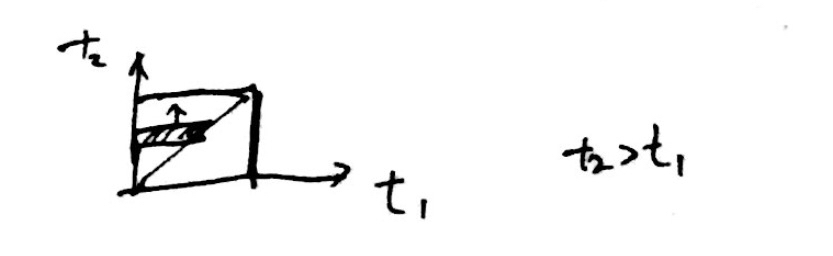
\includegraphics[width=1\textwidth]{figures/1.jpg}
		\caption{$t_2>t_1$}
	\end{figure}

    If we relabel $t_1$ to $t_2$, $t_2$ to $t_1$, we get:
    \begin{align} \label{eq:n_is_22} \int_{t_0}^{t}dt_1 \int_{t_0}^{t_1}dt_2 \cdot \hat{V}_I(t_1) \hat{V}_I(t_2)  
    \end{align}

    Then the integration is changed into:

	\begin{figure}[H]
		\centering
		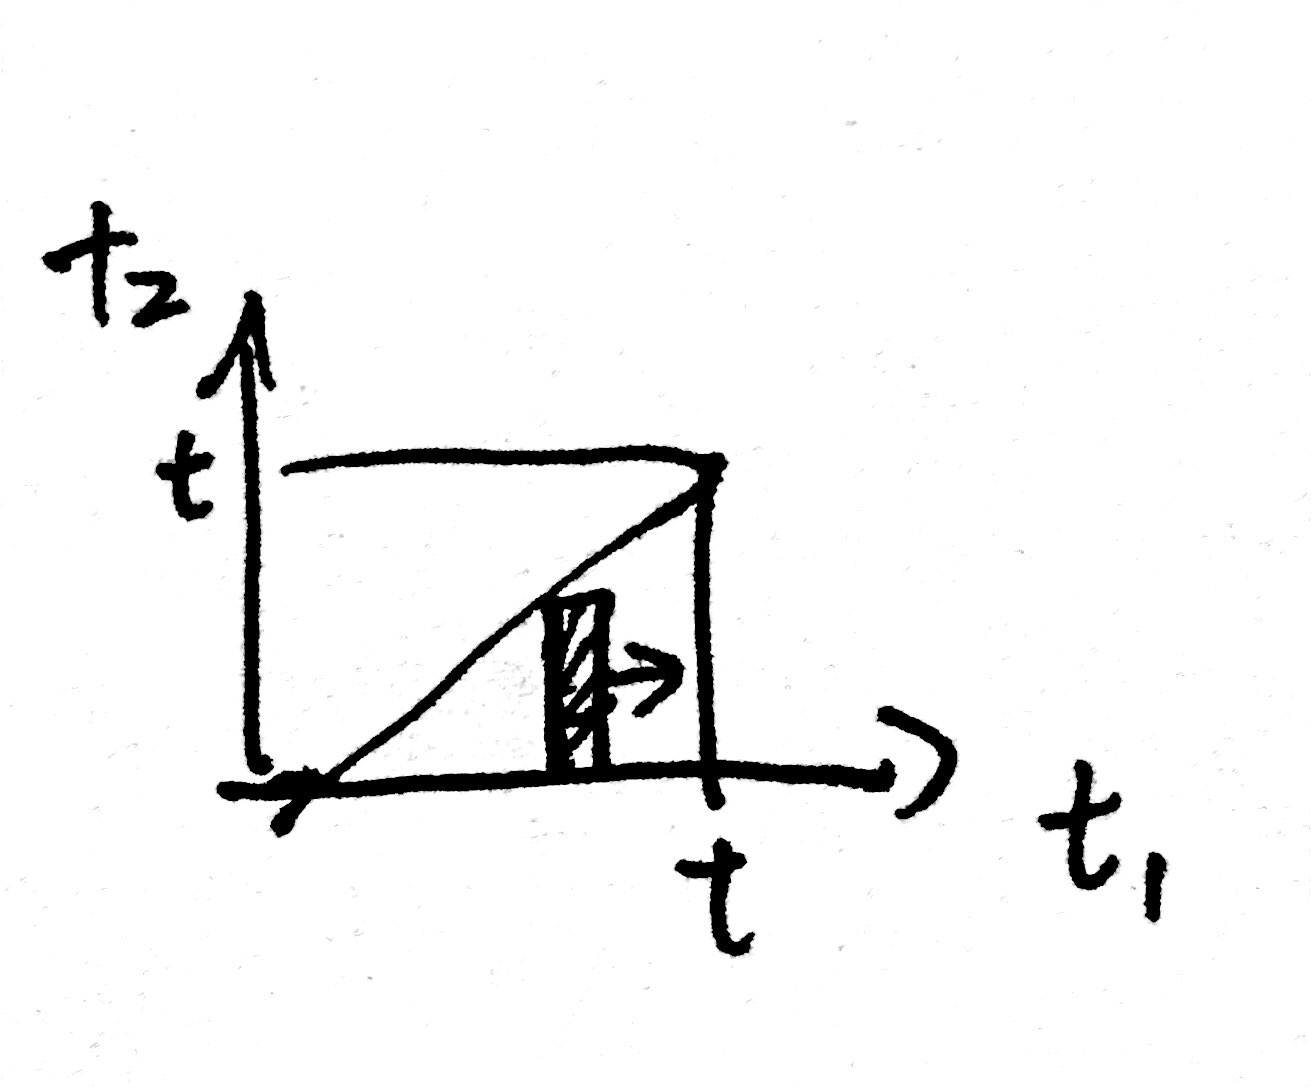
\includegraphics[width=0.8\textwidth]{figures/2.jpg}
		\caption{$t_1>t_2$}
	\end{figure}

    We observe that doing the two integration is equivalent to doing a full integral over the region marked by ($t_0 \leqslant t_1 \leqslant t $ and $t_0 \leqslant t_2 \leqslant t$),

	\begin{figure}[H]
		\centering
		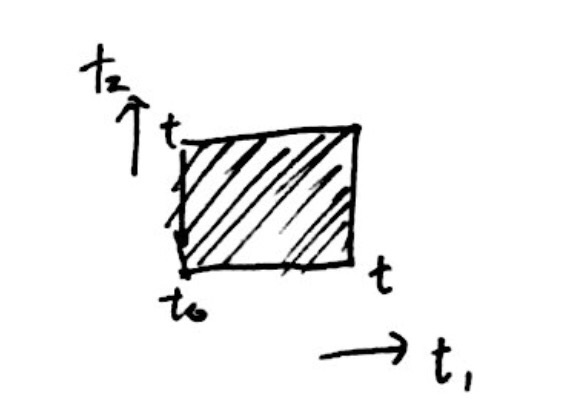
\includegraphics[width=0.6\textwidth]{figures/3.jpg}
		\caption{Whole region}
	\end{figure}

    while restricting the value of integration in the proper region and putting the operators in correct order.

    For example:
    
    \fref{eq:n_is_21} is: $\int_{t_0}^{t}dt_2 \cdot \int_{t_0}^{t_2} dt_1 \theta(t_1-t_2) \hat{V}_I(t_2) \hat{V}_I(t_1)$
    
    \fref{eq:n_is_22} is: $\int_{t_0}^{t}dt_1 \int_{t_0}^{t_1}dt_2 \cdot \theta(t_1-t_2) \hat{V}_I(t_2) \hat{V}_I(t_1)$
    
    where $\theta(t_1-t_2)$ is restricting the to region $t_2>t_1$. Also, I put the latest time in the front.
    
    \subsubsection{Time Ordering Operator T}
    
    We introduce a time ordering operator $T$ to signify the process we described above. When $T$ acts on a set of operators, it automatically sorts them in descending time order. 
    
    For example, if $t_3>t_2>t_1$, then
    
    $$T(A(t_1)B(t_3)C(t_2)) = B(t_3)C(t_2)A(t_1)$$
    
    Then
    
    \begin{align}
        \int_{t_0}^{t}dt_1 \int_{t_0}^{t}dt_2 =& T (\hat{V}(t_1) \hat{V}(t_2))
        \\
        = (\text{integration of } &\hat{V}_I(t_1) \hat{V}_I(t_2) \text{ when } t_1>t_2 ) \nonumber\\
         +(\text{integration of } &\hat{V}(t_2)\hat{V}(t_1) \text{ when } t_2>t_1)
        \nonumber\\
        = (\int_{t_0}^{t}dt_1 \int_{t_0}^{t_1}dt_2 & \hat{V}_I(t_1) \hat{V}_I(t_2)  \nonumber\\
        + (\int_{t_0}^{t}dt_2 \int_{t_0}^{t_2} dt_1 &\hat{V}_I(t_2) \hat{V}_I(t_1))
    \end{align}
    
    But \fref{eq:n_is_22} is equal to \fref{eq:n_is_21}, because $ \int_{t_0}^{t}dt_2 \cdot \int_{t_0}^{t_2} dt_1 \hat{V}_I(t_2) \hat{V}_I(t_1)= \frac{1}{2} \cdot \int_{t_0}^{t}dt_1 \int_{t_0}^{t}dt_2 \cdot T[\hat{V}_2(t_1) \hat{V}_2(t_2)]  $
    
    Similarly, for arbitrary n, we have
    $$ \int_{t_0}^{t}dt_n \int_{t_0}^{t_n}dt_(n-1) \cdots \int_{t_0}^{t}dt_1 \cdot 
    \hat{V}_I(t_n) \cdots \hat{V}_I(t_1)
    =\frac{1}{n!} \cdot \int_{t_0}^{t}dt_n \cdots \int_{t_0}^{t}dt_1 \cdot 
    T(\hat{V}_I(t_n) \cdots \hat{V}_I(t_1))
    $$
    
    The factor $n!$ is that we have in total $n!$ different ways to rearrange {$t_1,\cdots, t_n$}. And each arrangement {$t_{i_1}, \cdots,t_{i_n}$} corresponds to a region in ${[t_0, t_0]}^n$ where $t_0 \leqslant t_{i_1} < \cdots < t_{i_n} \leqslant t$.
    
    Thus we the most useful expression for operator $\hat{U}$:
    
   	\begin{align}
    	\hat{U}(t,t_0) = \sum_{n=0}^{\infty}
    	\frac{(-i)^n}{n!}
    	\int_{t_0}^{t} dt_1 \int_{t_0}^{t} dt_2
    	\dotsb \int_{t_0}^{t} dt_n
    	T[\hat{V}(t_1)\dotsb\hat{V}(t_{n})]
   	\end{align}

    \subsection{Adiabatic Switch on}
    
    The next idea for interacting many-body system is to use the notion of adiabatic switch on. In the Interaction Picture, we assume our Hamiltonian is:
    
    $$ H=H_0 +V $$
    
    We wish to extract the eigenstate of $H$ from that of $H_0$. Hence we imagine that we have 
    
    $$ H' = H_0 + e^{-\epsilon |t|}V  $$
    
    So we have $\lim_{t\to\infty} H'= \lim_{t\to\infty} H'=H_0 $.
    
    In this scenario, we have
    
    $$ \ket{\Psi(t=\pm\infty)} = \ket{\Phi_0}   $$
    
    where $\ket{\Phi_0}$ can be exactly solved.
    
    Then using the evolution operator $U$, we can bring up the states from $-\infty$ to now $t=0$.
    
    \begin{align}
        \ket{\Psi(t=0)} =& U_\epsilon (0,-\infty) \ket{\Psi(t=-\infty}
        \\
        =& U_\epsilon (0,-\infty) \ket{\Psi(\infty)}
    \end{align}
    
    This is the solution to $H=H_0+V$, since $e^{-\epsilon \cdot 0}=0$.
    
    %\marginpar Note How $e^{-\epsilon (t)}=0$
    
    However, there is a problem with this. Because the real physical system is in the Hamiltonian $H=H_0+V$ all the time. And our system dives in the Hamiltonian $H$ only at one instant of time. If the result of over calculation is to be meaningful, it must be independent on $\epsilon$.
    How
    In addition, we have a Gell-Mann and Low theorem, which requires a length proof provided in appendix \ref{appendix:Proof_of_G-M_Low}. It states that:
    
    If the following quantity exists to all orders in perturbation theory, (denoting $\ket{\Psi_0} :\equiv U_{\epsilon} (0, -\infty) \ket{\Phi_0}$. )
    
    	$$ \frac{\hat{U}_\epsilon(0,-\infty)\ket{\Phi_0}}{\bra{\Phi_0}\hat{U}_\epsilon(0,-\infty)\ket{\Phi_0}}
    	\equiv
    	\frac{\ket{\Psi_0}}{\braket{\Phi_0|\Psi_0}}
    	$$
    	then $\ket{\Psi_0}$ is an eigenstate of $\hat{H}$ in the following sense:
    	$$\hat{H}\frac{\ket{\Phi_0}}{\braket{\Phi_0|\Psi_0}}
    	=
    	E \frac{\ket{\Psi_0}}{\braket{\Phi_0 |\Psi_0}}
    	$$
    
    %If the following .....(pp. 61) of Fetter. 
    
    The equation (6.44) could be recast into a new form.
    
    $$\bra{\Phi_0} \hat{H} \frac{\ket{\Psi_0}}{\braket{\Phi_0|\Psi_0}}
    = E \cdot \frac{\braket{\Phi_0|\Psi_0}}{\braket{\Phi_0|\Psi_0}}
    $$
    
    Since $H=H_0+V$ and $\braket{\Phi_0|H_0|\Psi_0} = E_0 \cdot {\braket{\Phi_0|\Psi_0}}$, we have
    
    \begin{align} \frac{\braket{\Phi_0|V|\Psi_0}}{\braket{\Phi_0|\Psi_0}}= E-E_0   \label{eq:6.45}
    \end{align}
    
    Thus, in the limit $\epsilon \rightarrow 0$ we have a way to calculate the energy of our physical system's $E$ by \ref{eq:6.45}. This is also intuitively satisfying, since when $\epsilon$ is small, $\hat{H}'$ approximates $\hat{H}$ in a long enough time. If we imagine that we turn on $H'$ from $t=-\infty$ very slowly, then we are confident that our calculation is giving us the real wave function and its energy.
    

\section{Green Function}
\label{sec:Green Function}

\section{Todo}

Here lists I want to add to this article.

First I will define Green functions
\footnote{could be found on \cite{fetter} or \cite{mahan}},
which are related to a variety of physical phenomenons. Then the above idea of adiabatic switch on will allow me to give a formula for Green functions. I will show that this formula, combined with perturbative solution to $\hat{U}$ and the Wick's thoerem
\footnote{Proof of Wick's theorem could be found on \cite{fetter}},
gives us a systematical way of calculating Green functions. I will then explain Feynman Diagrams
\footnote{Both \cite{fetter} and \cite{mahan} explains Feynman Diagrams, though \cite{fetter} explains in more detail.}
, which will give a graphical representation of each Green functions. I will try to understand the new path integral way of calculating Feynman Diagrams\footnote{Could be found on \cite{Negele}.}.

%% ----------------------------------------------------------
%%                       TODO 
%% ----------------------------------------------------------
% 1. Change the bibligraphy into a modern style.
% 2. Improve the identation of source file
% 3. put \ref into \fref.
% 4. Explain for the g in the proof of \ref{appendix:Proof_of_G-M_Low}
% 5. Also in \ref{appendix:Proof_of_G-M_Low}, I think we should call it $\lim_{\epsilon\to 0^+} is finite!
% 6. Give a Mindmap for this article.
% 7. Solve those problems in \marginpar
%\section{Def. Single Particle Green function}
%%Sec 7. (ch3. Sec 3.7) Green Function
%
%$G_{\alpha \beta}$ be s.t.
%$$ iG_{\alpha \beta} (xt,x't')= 
%\frac{\braket{\Psi_0|T[\hat{\psi}_{H\alpha}(x,t)\psi_{H\beta}^{\dagger}(x',t)|\Psi_0}}
%{\braket{\Psi_0|\Psi_0}}  \text{  (7.1)of Fetter  }
%$$
%
%Here, $\ket{\Psi_0}$ and $\psi_H$ are in Heisenberg picture. $\alpha$ and $\beta$ index the spin.
%
%$T$ is defined differently as:
%
%% (7.4) of Fetter.
%
%But this is consistent with previous example, because
%% (under 7.4 of Fetter)
%
%\section{Reason for Green function}
%
%The usefulness of Green function could be demonstrated in several aspects. Although I will not go into the details, I will list three points.
%
%\begin{enumerate}
%	\item Green functions are related to a wide range of observations. To list a few, we have
%	$$(7.7), (7.8)(7.9)(7.10)(7.22)(7.32)
%	$$
%	\item Green functions can be interpreted as a Gredantoer experiment. For example, when $t>t'$, 
%	$$ iG_{\alpha \beta} (xt,x't')= 
%	\braket{\Psi_0|\hat{\psi}_{H\alpha}(x,t)\psi_{H\beta}^{\dagger}(x',t')|\Psi_0}
%	$$
%	%(6.31) of Fetter @ 59
%	
%	\begin{align}
%	\braket{\Psi_I(t)
%		|\hat{\psi}_{I\alpha}(x,t) \hat{U}(t,t') \psi_{I\beta}^{\dagger}(x',t')|
%		\Psi_I(t')}
%	=& \braket{\Phi_0|
%		\hat{U}(-\infty,t) \cdot \hat{U}(t,0) \psi_{H\alpha}(x,t) \hat{U}(0,t) \cdot \hat{U}(t,t') 
%		\times \hat{U}(t',0) \hat{\psi}_{H\beta}^{\dagger}(x',t') \hat{U}(0,t') \cdot \hat{U}(t',-\infty)
%		|\Phi_0}
%	\\
%	=& \braket{\Phi_0
%		|\hat{U}(-\infty,0) \hat{\psi}_{H\alpha}(x,t) \psi_{H\beta}^{\dagger}(x,t') \hat{U}(0,-\infty) |
%		\Phi_0}
%	\end{align}
%	
%	Thus the Green Function could be viewed as 
%	%pp.96 of Jrshi. Sec 6.2.
%	
%	\item There is particularly useful technique to calculate the Green function perturbatively, which is what we are going to illustrate in the next section, i.e. Feymann Diagram.
%\end{enumerate}
%
%\section{Feynman's Diagram and Wick's Theorem}
%
%%(Sec8 of Fetter)
%
%\subsection{alsdkfjlsdkjfal}
%{From \text{$\braket{\hat{O}_H}$} to \text{$\braket{\hat{O}_S}$|}
%	
%	Before applying perturbative analysis, we first need to transform the Green's function defined in Heisenberg picture into a more convenience form.
%	
%	\subsubsection{Theorem}
%	$$ \frac{\braket{\Psi_0 | \hat{O}_H(t) | \Psi_0}}
%	{\braket{\Psi_0 | \Psi_0}} 
%	=
%	\frac{1}{\cdots} 
%	%(8.1) of Fetter
%	$$
%	
%	where $S= \hat{U}_\epsilon (\infty,-\infty)$.
%	
%	$S$ is called the S-Matrix, because it relates the initial state and final state of the system.

% Eki finishes!
\appendix %See: http://www.tex.ac.uk/FAQ-appendix.html

\section{Proof of Gell-Mann and Low Theorem}
\label{appendix:Proof_of_G-M_Low}
The theorem states:

\begin{thm}
	If the following quantity exists to all orders in perturbation theory:
	
	$$ \frac{\hat{U}_\epsilon(0,-\infty)\ket{\Phi_0}}{\bra{\Phi_0}\hat{U}_\epsilon(0,-\infty)\ket{\Phi_0}}
	\equiv
	\frac{\ket{\Psi_0}}{\braket{\Phi_0|\Psi_0}}
	$$
	then $\ket{\Psi_0}$ is an eigenstate of $\hat{H}$ in the following sense:
	$$\hat{H}\frac{\ket{\Phi_0}}{\braket{\Phi_0|\Psi_0}}
	=
	E \frac{\ket{\Psi_0}}{\braket{\Phi_0 |\Psi_0}}
	$$
\end{thm}

Proof:

Here and afterwards, we will set $\ket{\Psi_0(\epsilon)} \equiv \hat{U}_\epsilon(0,-\infty) \ket{\Phi_0}$.

Consider the following:

\begin{align}
(\hat{H}_0-E_0) \ket{\Psi_0(\epsilon)} =& (\hat{H}_0 - E_0)\hat{U}_\epsilon(0,-\infty)\ket{\Psi_0} \\		
=& \left( \hat{H}_0 \hat{U}_\epsilon(0,-\infty) - \hat{U}_\epsilon(0,-\infty)E_0\right)  \ket{\Psi_0} \\
=& \left( \hat{H}_0\hat{U}_\epsilon(0,-\infty) - \hat{U}_\epsilon(0,-\infty) \hat{H}_0\right) \ket{\Psi_0} \\
=& [\hat{H}_0, \hat{U}_\epsilon(0,-\infty)] \ket{\Psi_0}
\label{eq:6.46}
\end{align}

The expression for $\hat{U}_\epsilon(0,-\infty)$ is explicitly:

\begin{align}
\hat{U}_\epsilon(0,-\infty) =& \nonumber\\
\sum_{n=0}^{\infty} \frac{(-i)^n}{n!} &\int_{-\infty}^{0} dt_1 \dotsb \int_{-\infty}^{0} dt_n e^{\epsilon(t_1+\dotsb+t_n)} T[\hat{V}(t_1)\dotsb \hat{V}(t_n)]
\end{align}

So we need $[\hat{H_0}, \hat{V}(t_1)\dotsb\hat{{V}(t_n)}]$ to get $[\hat{H}_0, \hat{U}_\epsilon(0,-\infty)]$.

\begin{lemma}
	$[H,ABC\dotsb] = \left( [H,A] BC\dotsb\right)  + \left( A[H,B]C\dotsb\right)  + \dotsb$
\end{lemma}

Proof:

Obviously we have: 
\begin{align}[H,AB] = [H,A]B + A[H,B] \label{eq:HAB}\end{align}
Then for more terms we can, for example:
\begin{align}
[H,ABC] =& [H,AB] C + AB[H,C] \nonumber\\
=& [H,A]BC + A[H,B]C + AB[H,C] \nonumber
\end{align}

Thus one may obviously obtain the lemma by using \fref{eq:HAB} recursively.

Using above lemma, one has:

\begin{align}
[\hat{H}_0,\hat{V}(t_1)\dotsb\hat{V}(t_n)] &= [\hat{H}_0,\hat{V}(t_1)]\hat{V}(t_2)\dotsb \nonumber\\
&+ \dotsb \nonumber \\
&+ \hat{V}(t_1)\dotsb\hat{V}(t_{n-1})[\hat{H}_0,\hat{V}(t_n)] 
\end{align}

Also, in Interaction Picture, one has:
$$ i\frac{\partial \hat{V}(t)}{\partial t} = [\hat{V}(t),\hat{H}_0]$$
or:
$$ \frac{1}{i} \frac{\partial \hat{V}(t)}{\partial t} = [\hat{H}_0,\hat{V}(t)]$$
Hence the above commutators are turned into partial derivatives:

\begin{align}
[\hat{H}_0,\hat{V}(t_1)\dotsb\hat{V}(t_n)] &= \frac{1}{i} \left( \frac{\partial}{\partial t_1} + \dotsb + \frac{\partial}{\partial t_n}  \right)  \hat{V}(t_1)\dotsb\hat{V}(t_{n})
\label{eq:eq_of_HVVV}
\end{align}

We need an additional fact:
\begin{align}
T[\left( \frac{\partial}{\partial t_1} + \dotsb + \frac{\partial}{\partial t_n}  \right)  \hat{V}(t_1)\dotsb\hat{V}(t_{n})] &= \left( \frac{\partial}{\partial t_1} + \dotsb + \frac{\partial}{\partial t_n}  \right)  T [\hat{V}(t_1)\dotsb\hat{V}(t_{n})]
\label{eq:partial_T}
\end{align}
This can be seen on an example. Notice that 
$T[\hat{V}(t_1)\hat{V}(t_2)] = \theta(t_1-t_2)\hat{V}(t_1)\hat{V}(t_2) + \theta(t_2-t_1)\hat{V}(t_2)\hat{V}(t_1)$, where $\theta(t)$ is Heaviside step function. We also have: $\frac{\partial}{\partial t}\theta(t) = \delta(t) $. So when $t_1\neq t_2$, $T\frac{\partial}{\partial t_1} = \frac{\partial}{\partial t_1} T$, i.e. it commutes with $T$. When $t_1 = t_2$, this is obviously also correct as well. Hence:
$$
T[ \frac{\partial}{\partial t_1} \hat{V}(t_1) \hat{V}(t_{2})] = 
\frac{\partial}{\partial t_1} T[  \hat{V}(t_1) \hat{V}(t_{2})]
$$
Similar arguments will give us \fref{eq:partial_T}, since $T$ is essentially a series of $\theta(t)$ functions.

Using the above fact and \ref*{eq:eq_of_HVVV}, one turns \ref*{eq:6.46} into (Denote $\int_{-\infty}^{0} dt_1\dotsb \int_{-\infty}^{0} dt_n$ as \textit{(Integrate)}):
\begin{align}
(\hat{H}_0-E_0)\ket{\Psi_0(\epsilon)} =& \nonumber\\
\Bigl[ 
\hat{H}_0, 1+\sum_{n=0}^{\infty} \frac{(-i)^n}{n!} 
&\text{\textit{ (Integrate) }}
e^{\epsilon(t_1+\dotsb+t_n)} T[\hat{V}(t_1)\dotsb \hat{V}(t_n)]
\Bigr] \nonumber\\
=& \sum_{n=1}^{\infty} \frac{(-i)^n}{i\cdot n!} 
\text{\textit{ (Integrate) }}
e^{\epsilon(t_1+\dotsb+t_n)} 
\left( \frac{\partial}{\partial t_1} + \dotsb + \frac{\partial}{\partial t_n}  \right) 
T[\hat{V}(t_1)\dotsb \hat{V}(t_n)] \nonumber\\
=& \sum_{n=1}^{\infty} - \frac{(-i)^{n-1}}{n!} 
\text{\textit{ (Integrate) }}
e^{\epsilon(t_1+\dotsb+t_n)}
\left( \frac{\partial}{\partial t_1} + \dotsb + \frac{\partial}{\partial t_n}  \right)
T[\hat{V}(t_1)\dotsb \hat{V}(t_n)]
\label{eq:6.46_2}
\end{align}

Integration by parts gives us, for example:

$$\int_{-\infty}^{0} dt_1 e^{\epsilon t_1} \frac{\partial}{\partial t_1} T[\hat{V}(t_1)] 
= 
e^{\epsilon t_1} T[\hat{V}(t_1)] \bigg|_{\infty}^0 - \epsilon\int_{\infty}^{0} dt_1 e^{\epsilon t_1}T[\hat{V}(t_1)]$$

Similarly:
\begin{align}
&\text{\textit{ (Integrate) }}
e^{\epsilon(t_1+\dotsb+t_n)}
\frac{\partial}{\partial t_1}
T[\hat{V}(t_1)\dotsb \hat{V}(t_n)] \nonumber \\
&= \hat{V}(0) \text{\textit{ (Integrate without $t_1$) }} 	e^{\epsilon(t_2+\dotsb+t_n)}
T[\hat{V}(t_2)\dotsb \hat{V}(t_n)] \nonumber \\
&- \epsilon \text{\textit{ (Integrate) }}
e^{\epsilon(t_1+\dotsb+t_n)}
T[\hat{V}(t_1)\dotsb \hat{V}(t_n)]
\end{align}

For other "$\frac{\partial}{\partial t_i}$", the procedure is essentially the same, and they all contribute to the same value, as can be seen by relabeling the dummy indices "$t_1 \dotsb t_n$". Hence \ref{eq:6.46_2} is:

\begin{align}
(\hat{H}_0-E_0)\ket{\Psi_0} &= 
\sum_{n=1}^{\infty} - \frac{(-i)^{n-1}}{n!} \cdot n \times \nonumber \\
&\bigg\{
\hat{V}(0) \text{\textit{ (Integrate without $t_1$) }}
e^{\epsilon(t_2+\dotsb+t_n)}
T[\hat{V}(t_2)\dotsb \hat{V}(t_n)] \nonumber\\
&-
\epsilon
\text{\textit{ (Integrate) }}
e^{\epsilon(t_1+\dotsb+t_n)}
T[\hat{V}(t_1)\dotsb \hat{V}(t_n)]	
\bigg\}
\ket{\Phi_0}  \nonumber \\
&\text{($n$ for $n$ same contributions from 
	$\int_{-\infty}^{0} dt_1 \dotsb \int_{-\infty}^{0} dt_n$.)} \nonumber\\
&= -\hat{V}(0)\hat{U}_\epsilon(0,-\infty) \ket{\Phi_0}
\text{(the first term)} \nonumber\\
&+ \epsilon \sum_{n=1}^{\infty} \frac{(-i)^{n-}}{(n-1)!}
\text{\textit{ (Integrate) }}
e^{\epsilon(t_1+\dotsb+t_n)}
T[\hat{V}(t_1)\dotsb \hat{V}(t_n)] \ket{\Phi_0} \nonumber
\end{align}
The second term is dealt with as follows:
\begin{align}
\frac{(-i)^{n-1}}{(n-1)!} \text{\textit{ (Integrate) }} 
T[\hat{V}(t_1)\dotsb \hat{V}(t_n)] & 
\text{(assuming $\hat{V} = g\cdot \hat{V}')$} \nonumber\\
= \frac{(-i)^{n-1}}{(n-1)!} &\text{\textit{ (Integrate) }}
g^n T[\hat{V}'(t_1)\dotsb \hat{V}'(t_n)] \nonumber \\
=ig\frac{\partial}{\partial g} \frac{(-i)^n}{n!}g^n
&\text{\textit{ (Integrate) }} T[\hat{V}'(t_1)\dotsb \hat{V}'(t_n)]
\nonumber \\
=ig\frac{\partial}{\partial g} \frac{(-i)^n}{n!}g^n
&\text{\textit{ (Integrate) }} T[\hat{V}(t_1)\dotsb \hat{V}(t_n)]\nonumber
\end{align}
Hence:
\begin{align}
\text{second term} &= \epsilon
\sum_{n=1}^{\infty}ig \frac{\partial}{\partial g}
\frac{(-i)^n}{n!}
\text{\textit{ (Integrate) }} T[\hat{V}(t_1)\dotsb \hat{V}(t_n)] \ket{\Phi_0} \nonumber\\
&= i\epsilon g \frac{\partial}{\partial g}
\sum_{n=0}^{\infty}
\frac{(-i)^n}{n!}
\text{\textit{ (Integrate) }} T[\hat{V}(t_1)\dotsb \hat{V}(t_n)] \ket{\Phi_0} \nonumber\\
&\text{\quad(since $\frac{\partial}{\partial g}
	\text{(zeroth term)}=0$)} \nonumber\\
&=i\epsilon g \frac{\partial}{\partial g}
\hat{U}_\epsilon(0,-\infty) \ket{\Phi_0} \nonumber\\
&= i\epsilon g \frac{\partial}{\partial g} \ket{\Psi_0(\epsilon)}
\nonumber
\end{align}
Together we have (noting that $\hat{V}(0)$ is actually the interacting part of real Hamiltonian $\hat{V}$):
\begin{align}
(\hat{H}_0-E_0)\ket{\Psi_0(\epsilon)} = -\hat{V}\ket{\Psi_0(\epsilon)} + i\epsilon \frac{\partial}{\partial g} \ket{\Psi_0(\epsilon)}
\end{align}
Write it in another way:
\begin{align}
(\hat{H}_0+\hat{V}-E_0) \ket{\Psi_0(\epsilon)} &= (\hat{H} -E_0)\ket{\Psi_0(\epsilon)} \nonumber\\
&= i\epsilon g \frac{\partial}{\partial g} \ket{\Psi_0(\epsilon)}
\label{eq:6.50}
\end{align}
Multiplying left with
$\frac{\bra{\Phi_0}}{\braket{\Phi_0|\Psi_0(\epsilon)}}$,
we have:
\begin{align}
RHS &= i\epsilon g
\frac{
	\braket{\Phi_0|\frac{\partial}{\partial g} |\Psi_0(\epsilon)}
}
{\braket{\Phi_0|\Psi_0(\epsilon)}
}\nonumber\\
&\text{\quad(since 
	$\frac{\partial}{\partial g} \bra{\Phi_0}=0$)}\nonumber\\
&= i\epsilon g
\frac{
	\frac{\partial}{\partial g}\braket{\Phi_0|\Psi_0(\epsilon)}
}
{
	\braket{\Phi_0|\Psi_0(\epsilon)}
}\nonumber\\
&=i \epsilon g \frac{\partial}{\partial g}
\ln\braket{\Phi_0|\Psi_0(\epsilon)}
\end{align}
while:
\begin{align}
LHS = \frac{
	\braket{\Phi_0|\hat{H} | \Psi_0(\epsilon)}
}{
\braket{\Phi_0|\Psi_0(\epsilon)}
}
= E-E_0
\end{align}
So we have:
\begin{align} i \epsilon g \frac{\partial}{\partial g}
\ln\braket{\Phi_0|\Psi_0(\epsilon)} = E-E_0 
\label{eq:6.51}
\end{align}
From above expression, we notice that 
$\lim_{\epsilon\to 0^+} \epsilon \ln\braket{\Phi_0|\Psi_0(\epsilon)}$ is finite, otherwise we would have $E=E_0$ when $\epsilon\to 0^+$, which is absurd. Hence, $ln \braket{\Phi_0| \Psi_0(\epsilon)} \propto \frac{1}{\epsilon}$, or $\braket{\Phi_0| \Psi_0(\epsilon)} \propto e^{1/\epsilon}$.

Now we calculate

\begin{align}
&(H-E_0 - i\epsilon g \frac{\partial}{\partial g}) \frac{\ket{\Psi_0(\epsilon)}}
{\braket{\Phi_0|\Psi_0(t)}} \nonumber\\
&= \frac{
	(\hat{H}-E_0-i \epsilon g \frac{\partial}{\partial g})
	\ket{\Psi_0(\epsilon)}
}{
\braket{\Phi_0|\Psi_0(\epsilon)}
}
+ i\epsilon g
\frac{
	\ket{\Psi_0(\epsilon)}\frac{\partial}{\partial g}
	\braket{\Phi_0|\Psi_0(\epsilon)}
}{
\braket{\Phi_0|\Psi_0(\epsilon)}^2
} \nonumber\\
&= \text{(by \ref{eq:6.50} the first term vanishes)\quad} 0
+ \frac{\ket{\Psi_0(\epsilon)}}
{\braket{\Phi_0|\Psi_0(\epsilon)}}
\cdot
i \epsilon g \frac{\partial}{\partial g}
\ln\braket{\Phi_0|\Psi_0(\epsilon)} \nonumber\\
&= \text{(by \ref{eq:6.51})\quad}
\frac{\ket{\Psi_0(\epsilon)}}
{\braket{\Phi_0|\Psi_0(\epsilon)}}
\cdot
(E-E_0)
\end{align}
That is:
\begin{align}
\left( \hat{H} - E - i \epsilon g \frac{\partial}{\partial g}\right) 
\frac{\ket{\Psi_0(\epsilon)}}
{\braket{\Phi_0|\Psi_0(\epsilon)}}
= 0
\end{align}
Now by assumption 
$\frac{\ket{\Psi_0(\epsilon)}}
{\braket{\Phi_0|\Psi_0(\epsilon)}}$ is finite when 
$\epsilon\to 0^+$,
we have:
\begin{align}
\hat{H}\frac{\ket{\Phi_0}}{\braket{\Phi_0|\Psi_0}}
=
E \frac{\ket{\Psi_0}}{\braket{\Phi_0 |\Psi_0}}
\end{align}

\textbf{Q.E.D.}


\begin{thebibliography}{1}

	
	\bibitem{blog} \url{http://we-taper.github.io/}
	
	\bibitem{fetter} Alexander L. Fetter, John Dirk Walecka, Quantum Theory of Many-Particle Systems
	
	\bibitem{mahan}  Gerald D. Mahan, Many-Particle Physics (3rd)
	
	\bibitem{wiki:Plank_units} \url{https://en.wikipedia.org/wiki/Planck_units}
	(accessed June 1, 2016).
	
	\bibitem{Negele} Negele \& Orland, Quantum Many-particle Systems.
	
	
\end{thebibliography}


\section{License}
The entire content of this work (including the source code
for TeX files and the generated PDF documents) by 
Hongxiang Chen (nicknamed we.taper, or just Taper) is
licensed under a 
\href{http://creativecommons.org/licenses/by-nc-sa/4.0/}{Creative 
Commons Attribution-NonCommercial-ShareAlike 4.0 International 
License}. Permissions beyond the scope of this 
license may be available at \url{mailto:we.taper[at]gmail[dot]com}.

\end{document}
